\documentclass{paper}
\usepackage{subcaption}

\title{Chemistry IA}
\author{Chrtistoffer Corfield Aakre }

\begin{document}

\maketitle

\pagebreak

\section{Light polarisation}

All electromagnetic waves, such as visible light, oscillate in an infinite number of planes, each perpendicular to the direction of energy transfer. If the light passes through a \textbf{polarisation filter}, then the light will be \textbf{plane-polarised}: That is, it will only oscillate in the plane parallel to the plane of polarisation of the polarisation filter. See the figure below:

\begin{figure}[H]
\label{fig:polarisation}
\caption{Polarisation of light}
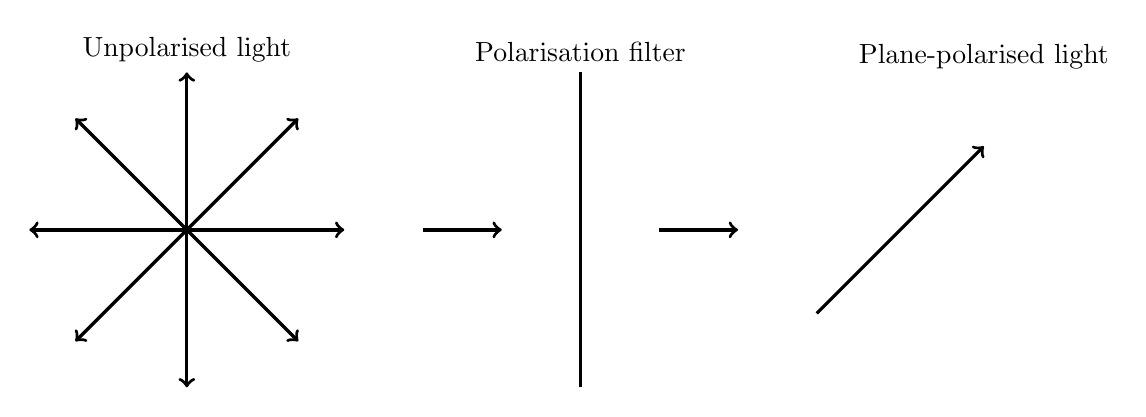
\begin{tikzpicture}

\draw[->, very thick] (0, 0) -- (0, 2) node[above]{Unpolarised light};
\draw[->, very thick] (0, 0) -- (0, -2);

\draw[->, very thick] (0, 0) -- (-2 / 1.414, 2 / 1.414);
\draw[->, very thick] (0, 0) -- (2 / 1.414, -2 / 1.414);

\draw[->, very thick] (0, 0) -- (-2 / 1.414, -2 / 1.414);
\draw[->, very thick] (0, 0) -- (2 / 1.414, 2 / 1.414);

\draw[->, very thick] (0, 0) -- (2, 0);
\draw[->, very thick] (0, 0) -- (-2, 0);

\draw[->, very thick] (3, 0) -- (4, 0);

\draw[very thick] (5, -2) -- (5, 2) node[above]{Polarisation filter};

\draw[->, very thick] (6, 0) -- (7, 0);

\draw[->, very thick] (8, -1.5 / 1.414) -- (8 + 3 / 1.414, 1.5 / 1.414) node[above, yshift=24pt]{Plane-polarised light};

\end{tikzpicture}
\end{figure}

\subsection{Intensity of a wave after polarisation}
Consider an electromagnetic wave with electric field $\vec{E}$ makes an angle $\theta$ with the transmission axis of a polarisation filter. Only the component of $\vec{E}$ that is along the transmission will pass through the polarisation filter. So, the component that passes through will be $\vec{E}\cos\theta$. We know from Physics that the intensity of an electromangetic wave is proportional to the square of the amplitude of its eletric field, so the intensity $I$ of the wave after passing through the filter will be given by

\begin{equation*}
    I = I_0\cos^2\theta,
\end{equation*}

where $I_0$ is the intensity of the wave before passing through the filter.

\subsection{Polarisation of unpolarised light}

If we shine unpolarised light through a polarisation filter, then we can calculate the new intensity by finding the \textbf{average} value of $I_0\cos^2\theta$:

\begin{align*}
    I &= \frac{I_0}{2\pi}\int_0^{2\pi} \cos^2\theta \; d\theta \\
    &= \frac{I_0}{2\pi}\int_0^{2\pi}\frac{\cos(2\theta) - 1}{2} \; d\theta \\
    &= \frac{I_0}{2\pi}\left(\frac{1}{4}\sin(2\theta) - \frac{1}{2}\theta\right)\Bigg\lvert_0^{2\pi} \\
    &= \frac{I_0}{2\pi}\left(0 - \frac{1}{2} \times 2\pi - 0 + 0\right) \\
    &= \frac{I_0}{2\pi} \times \frac{1}{2} \times 2\pi \\
    &= \frac{I_0}{2}.
\end{align*}

So, if we shine unpolarised light through a polarisation filter, then half the light will pass through, regardless of the filter's transmission axis.

\subsection{Interactions between polarisation filters}
While one polarisation filter on its one may not be too interesting, they can interact with each other in interesting ways. Below we consider two scenarios.

\subsubsection{Two perpendicular polarisation filters}
Now, let us shine light through two polarisation filters whose transmission axes are perpendicular to each other, like in the figure below; the angle between transmission axes and the initial polarisation of the light are shown above the polarisation filters, and the intensity of the wave is shown below each arrow:

\begin{figure}[H]
\label{fig:perpendicular-transmission-axes}
\caption{Two polarisation filters with perpendicular transmission axes}
\begin{tikzpicture}

\draw[->, very thick] (0, 0) -- (2, 0) node[midway, yshift=-50pt]{$I_0$};

\draw[very thick] (3, -2) -- (3, 2) node[above]{$\alpha$};

\draw[->, very thick] (4, 0) -- (6, 0) node[midway, yshift=-50pt]{$I_0\cos^2\alpha$};

\draw[very thick] (7, -2) -- (7, 2) node[above]{$\alpha + \pi/2$};

\draw[->, very thick] (8, 0) -- (10, 0) node[midway, yshift=-50pt]{$I_0\cos^2\alpha\cos^2(\pi / 2)$};

\end{tikzpicture}
\end{figure}

Of course, $\cos^2(\pi / 2) = 0$, so the intensity will be zero after the second polarisation filter.

\subsubsection{Adding a third polarisation filter}
Now, we please a third polarisation filter in between the first two, and repeat the experiment:

\begin{figure}[H]
\label{fig:third-filter}
\caption{Adding a third filter}

\begin{tikzpicture}

\draw[->, very thick] (0, 0) -- (2, 0) node[midway, yshift=-50pt]{$I_0$};

\draw[very thick] (3, -2) -- (3, 2) node[above]{$\alpha$};
'
\draw[->, very thick] (4, 0) -- (6, 0) node[midway, yshift=-50pt]{$I_0\cos^2\alpha$};

\draw[very thick] (7, -2) -- (7, 2) node[above]{$\alpha + \beta$};

\draw[->, very thick] (8, 0) -- (10, 0) node[midway, yshift=-50pt]{$I_0\cos^2\alpha\cos^2(\beta)$};

\draw[very thick] (11, -2) -- (11, 2) node[above]{$\alpha + \pi/2$};

\draw[->, very thick] (12, 0) -- (14, 0) node[midway, yshift=-50pt, xshift=25pt]{$I_0\cos^2\alpha\cos^2\beta\cos^2(\pi / 2 - \beta)$};

\end{tikzpicture}
\end{figure}

So, adding a third filter actually allowed some light to pass through when it would otherwise not.

\section{Stereoisomerism}

\textbf{Stereoisomers} are molecules where the atoms are in the same order, but the spatial arrangment of the atoms is different. We have four different types of stereoisomerism:

\begin{boldenumerate}
\item \textbf{Configurational isomers} can be \Quote{swapped} by breaking covalent bonds.
\item \textbf{Conformational isomers} can be obtained by rotating about $\sigma$ bonds.
\item \textbf{cis-trans and E/Z isomers} have restricted rotation about the atoms
\item \textbf{Optical isomers} have chiral carbon atoms.
\end{boldenumerate}

For this investigation, we will only concern ourselves with optical isomers.

\subsection{Optical isomers}
If a carbon attom is bonded to four \textit{different} atoms or groups, we call it a \textbf{chiral} carbon atom. Below are some examples of chiral carbon atoms, shown in blue:

\begin{figure}[H]
\label{fig:chiral-carbon-atoms}
\caption{Examples of chiral carbon atoms}
\begin{subfigure}[t]{.49\textwidth}
\centering
\chemfig{ H - \textcolor{blue}{C}([:90] - CH_3)([:-90] - F)-Cl} 
\end{subfigure}
\begin{subfigure}[t]{.49\textwidth}
\centering
\chemfig{H_3C - \textcolor{blue}{C}([:90] - OH)([:270] - H) - C([:45] = O)([:-45] - OH)} 
\end{subfigure}

\vspace{25pt}

\begin{subfigure}[t]{.49\textwidth}
\centering
\chemfig{H - C([:90] - H)([:-90] - H) - \textcolor{blue}{C}([:90] - H)([:-90] - Br) - CH_3} 
\end{subfigure}
\begin{subfigure}[t]{.49\textwidth}
\centering
\chemfig{\textcolor{blue}{C}([:225] - HO_2C)([:90] - CH_3)([:-5] <: H)([:-45] < OH)} 
\end{subfigure}


\end{figure}

The four groups are arranged tetrahedally around the chiral carbon atom, like below:

\begin{figure}[H]

\chemfig{
@1C([:225] <: @2H)([:90] - @3Br)([:-45] - @4CH_3)([:-95.5] < @5OH)
}

\end{figure}

and the bond angle is $109.5 \degree$. Optical isomers can be arranged in two different ways, each a mirror image of the other. These isomers are given ($+$) and ($-$) prefixes. See the figure below:

\begin{figure}[H]
\label{fig:fructose-optical-isomers}
\caption{Optical isomers of fructose}

\begin{subfigure}[H]{.49\textwidth}
\caption{($+$) Fructose}
\centering
\chemfig{[:-90]
CH_2OH - C([::90] = 0) - C^{\textcolor{orange}{3}}([::90] - H)([::-90] - HO) - C^{\textcolor{orange}{4}}([::90] - OH)([::-90] - H) - C^{\textcolor{orange}{5}}([::90] - OH)([::-90] - H) - CH_2OH
}
\end{subfigure}
\begin{subfigure}[H]{.49\textwidth}
\caption{($-$) Fructose}
\centering
\chemfig{[:-90]
CH_2OH - C([::90] = 0) - C^{\textcolor{orange}{3}}([::90] - OH)([::-90] - H) - C^{\textcolor{orange}{4}}([::90] - H)([::-90] - HO) - C^{\textcolor{orange}{5}}([::90] - H)([::-90] - HO) - CH_2OH
}
\end{subfigure}
\end{figure}

Such mirror images are called \textbf{enantiomers}. If a mixture contains equal amounts of each enantiomer, it is called a \textbf{racemate}, and is optically inactive. That is, it does not polarise light. However, if the mixture contains mostly one enantiomer, such as ($-$) fructose, then we would expect it to polarise light.

\end{document}
